\section{Local systems on a presented groupoid}
\label{sec:forest}
A finite graph can present a category with infinitely many arrows. As a simple example, one invertible generator at one vertex and no relators presents the group of integers. Enumerating a finite category table would miss this example. Instead we compute with transports of finite fibres. This also gives an exact test for when locally consistent choices of branches fit together around a loop.

\paragraph{The presentation.}
Take vertices $v<V$, generating directed edges $e<E$ with source $s(e)$ and target $t(e)$, and a finite list of pairs of parallel, composable words in signed edges. A positive letter traverses its edge forward and a negative letter backward. A path is a start vertex and a finite valid word, so the empty path has a specified base. Arrows of the presented groupoid are paths modulo the congruence generated by inverse cancellations and the listed word pairs. The following constructions do not require deciding equivalence of two paths.

A finite local system $A$ specifies a natural number $d_v$ at each vertex and a bijection $A_e:[d_{s(e)}]\to[d_{t(e)}]$ at each edge, where $[d]=\{0,\ldots,d-1\}$. Store the forward and inverse tables and verify both inverse equations. $A_p$ is successive lookup along a word $p$, with the inverse table for a negative letter. Require $A_p=A_q$ for each listed pair $(p,q)$, tested at every element of its source. Composition of paths then acts by composition of tables. Cancelling adjacent inverse letters preserves the result at any entry. Applying a listed pair inside a context preserves it, since equal intermediate entries give the same entries after the remaining suffix. Given a chain of such replacements, induction on its coded length proves equality of evaluations. This proves soundness for the presented groupoid even if its word problem is undecidable. A morphism $A\to B$ consists of tables $h_v:[d_v^A]\to[d_v^B]$ with $h_t A_e=B_e h_s$. Composing with inverses yields the equation for negative edges; induction along a supplied word gives it for every path.

\paragraph{Choosing the forest.}
Process a bounded array of marked vertices, initially empty. If there is an edge with exactly one marked endpoint, choose the first such edge, give its unmarked endpoint the same root, and record the signed edge from parent to child. Otherwise start a new root at the least unmarked vertex. Stop after $V$ markings. A completed component has no edge to an unmarked vertex when a new root starts. Subsequently its vertices and neighbours are unchanged. In more detail, throughout marking there are no edges between distinct marked components, and every component except the currently growing one has no edge to the unmarked vertices. An extension from the current component preserves both assertions, and starting a root is allowed precisely when every marked component satisfies the latter assertion. These are bounded tests on the vertex and edge arrays. Thus both endpoints of every edge have the same root. The marking time strictly decreases along parent pointers, so following parents for at most $V$ steps gives a path from the root to any $v$, in reverse order. Denote the forward path by $P_v$ and put $T^A_v=A_{P_v}$. At a root $r$, $T^A_r$ is the identity.

For an edge $e:s\to t$ write
\[
             M^A_e=(T^A_t)^{-1} A_e T^A_s .
\]
This is a permutation of the root fibre. For a forest edge $M_e$ is the identity, irrespective of the generator's orientation. Indeed transport to the child is transport to the parent followed by that signed edge. For an arbitrary edge this table records the transport around the loop $P_s$, $e$, $P_t^{-1}$.

\begin{theorem}[Forest coordinates for local systems]\label{thm:forest}
Fix the computed forest of a finite groupoid presentation.
\begin{enumerate}
\item Finite local systems are equivalent, as a category, to systems consisting of one finite fibre per root and one permutation per nonforest edge, satisfying the original relators with forest letters set to the identity. Morphisms in the latter category are root-fibre maps intertwining these permutations.
\item Restriction to roots and extension along $T_v$ give inverse bijections between global sections of $A$ and tuples of elements $a_r$ satisfying $M^A_e(a_r)=a_r$ at every nonforest edge in component $r$. In particular the exact number of global sections is the product, over components, of their common fixed-point counts.
\end{enumerate}
The reductions, inverse constructions and all tests on the displayed finite data are uniformly primitive recursive.
\end{theorem}

\begin{proof}
Multiplying the expressions for $M_e$ along a valid path $p:u\to v$ cancels the intermediate $T$'s, giving $(T_v^A)^{-1}A_pT_u^A$. For reversed edges use the inverse permutation. The assertion follows also by induction on a word, keeping the start and current vertex and the accumulated finite table. The result for parallel relators proves that $A\mapsto (d_r^A,M_e^A)$ is well defined.

Let $h:A\to B$ be a morphism. Its path equation gives $h_vT_v^A=T_v^B h_r$. Therefore the root maps $k_r=h_r$ obey
\begin{equation}
                    k_r M^A_e=M^B_e k_r. \label{eq:intertwine}
\end{equation}
Conversely, given root tables satisfying \eqref{eq:intertwine} on nonforest edges, put
\[
                    h_v=T_v^B k_r (T_v^A)^{-1}.
\]
For every edge \eqref{eq:intertwine} holds, since on forest edges both permutations are identities. Multiplying \eqref{eq:intertwine} on the left by $T_t^B$ and on the right by $(T_s^A)^{-1}$ gives $h_tA_e=B_eh_s$. These constructions are mutual inverses on morphisms, and preserve identities and composites by cancellation. Given root data, extend it by using the root fibre at every vertex of its component, assigning identity on forest edges and the supplied permutations elsewhere. The relator test is exactly the stipulated one. Reduction of this extension returns the identical root data. Extension after reduction is isomorphic to the original system by the component maps $T_v^A$; the equation $T_t^A M^A_e=A_e T_s^A$ is their naturality, and $h_vT_v^A=T_v^B h_r$ gives naturality with respect to $h$. This proves the equivalence without invoking a skeleton-selection principle.

A section is a morphism from the constant singleton system. Its value at a root is one element $a_r$. Equation \eqref{eq:intertwine} is precisely the fixed-point condition. Extension gives $a_v=T_v^A(a_r)$. The root choices are independent across components, proving the product formula. The empty graph gives one empty section. An empty root fibre in a nonempty component gives zero sections.
\end{proof}

\paragraph{Arithmetic cost and quantifiers.}
The graph, words, local systems, witnesses of rewrites, and morphism tables are all numerical inputs. For a fixed presentation and two systems, \eqref{eq:intertwine} uses at most $\sum_{e<E}d_{r(e)}^A$ entry comparisons. To list \emph{all} root morphisms test at most $\prod_r(d_r^B)^{d_r^A}$ tables, with $0^0=1$. No loop scans the arrows of the presented groupoid. Word evaluation is primitive recursion on its supplied length. A concatenation or a context replacement can be checked at each of finitely many entries. The table validity, forest invariant, equality of composite tables, and fixed-point counts are bounded numerical predicates. For example, in the telescoping proof the invariant for a word prefix of length $i$ checks its current transport at every root entry below $d_r$ against the corresponding conjugated prefix table. Thus quantifier-free induction suffices after Booleanizing the finite tests. Soundness for a derivable path equation quantifies over an arbitrary \emph{given} rewrite chain after proving that its numerical evaluation is invariant. This use of the category is meaningful beyond finite arrow tables. It gives no procedure for distinguishing arbitrary unequal arrows by finite local systems.

\subsection{Why simple roots can fail to admit a global label}
Use the Euclidean complex modulus in this example. Consider the piecewise linear complex path $w$ on $[0,1]$ joining $1$ to $i$ to $-1$ at times $0,1/2,1$. The polynomial family
\[
                          Y^2-z(t),\qquad z(t)=w(t)^2
\]
starts and ends at the same polynomial. If $u$ is the linear coordinate on either half, $|w(t)|^2=(1-u)^2+u^2\ge1/2$. There are two simple roots $w(t),-w(t)$ separated by more than one throughout the loop. Continuing along the two halves and comparing the final fibre with the initial one exchanges the labels. In forest coordinates there is one nonforest generator with the transposition on $[2]$, whose fixed-point count is zero. The transition tables here have a direct analytic justification.

\begin{figure}[ht]
\centering
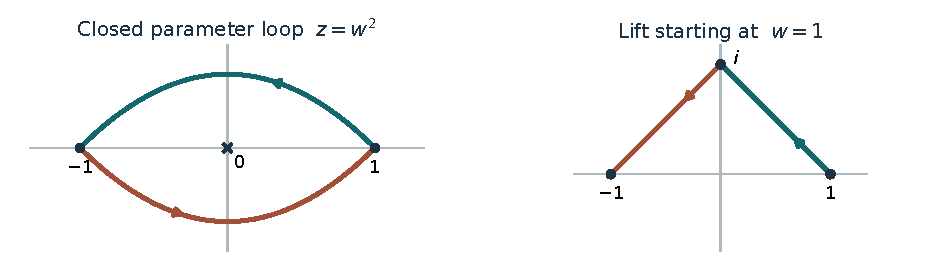
\includegraphics[width=.87\linewidth]{figures/square_root_lift.pdf}
\caption{Each color denotes one half of the parameter interval. The squared path closes at $1$. Its lift ends at $-1$ and therefore cannot give a section over the closed loop.}
\label{fig:lift}
\end{figure}
Suppose a root $y(t)$ along this loop is supplied at dyadic times by regular complex names, with a modulus ensuring that sufficiently close times give values at distance $\le1/4$. At each sampled time at least one of $|y-w|,|y+w|$ exceeds $1/2$, since their sum is at least $2|w|\ge\sqrt2$. Comparing approximations with sufficiently small fixed error (say $1/32$) identifies a factor with norm provably greater than $1/4$. In $(y-w)(y+w)=0$ this factor is invertible with an explicit norm lower bound, so the other is zero. This gives a PR sign bit at the sample, with a proof that $y$ is the indicated root; an input name here is a fixed PR family or a finite-demand parameter as specified in the framework. Choose a uniform dyadic grid whose mesh is at most $1/16$ and is within the supplied modulus at tolerance $1/4$. The path $w$ is $3$-Lipschitz, so adjacent $w$'s differ by $<1/4$. Opposite bits at adjacent samples $j,j+1$ would imply
\[
  2|w_j|\le |w_j+w_{j+1}|+|w_j-w_{j+1}|
            = |y_j-y_{j+1}|+|w_j-w_{j+1}|\le1/2.
\]
Thus adjacent bits agree. Induction is on bit equality with the first bit, and uses no unbounded extensional equality of complex names as its induction predicate. At the two endpoints the bit is the same and $w$ has changed sign, so $y(1)=-y(0)$, whereas $y(0)^2=1$. A periodic root label is impossible. This example distinguishes the existence of local analytic sheets with explicit separation from their compatibility on a loop. The finite test applies to a general analytic family once the charts and overlap transports have been justified. It does not derive those charts for arbitrary computable coefficients.

\subsection{Effective stable images in inverse towers}
\label{sec:stable-image}
The repository's categorical descent report exhibits a tower with PR-inhabited levels and no computable coherent point, and gives a construction when every bonding map is surjective. There is a useful intermediate hypothesis for towers with dead ends.

Let $A_n=\{x<b(n):V(n,x)=1\}$ be a fixed PR table family and $p_n:A_{n+1}\to A_n$ a fixed PR family of maps with a proof of typing. For $m\ge n$, let $p_{n,m}$ be the composite down from level $m$, with $p_{n,n}=1$. Suppose $h$ is a specified nondecreasing PR function with $h(n)\ge n$. Compute by bounded image search
\[
       I_n=p_{n,h(n)}(A_{h(n)}).
\]
Write $J(n,m)=p_{n,m}(A_m)$ and let $C(n)$ be the finite equality $p_n(I_{n+1})=I_n$. Given the inputs for a particular $n$, $C(n)$ is decidable by a PR test.

\begin{theorem}[Testing a proposed stable-image horizon]\label{thm:stable}
Under the preceding conditions, iPRA proves the equivalence
\[
 (\forall n\, C(n))\quad\longleftrightarrow\quad
 (\forall n\,\forall m\ge h(n)\; J(n,m)=I_n).
\]
If these conditions hold, there is a fixed PR producer which, given $a\in I_n$, extends $a$ to an infinite coherent tail in the sense of a PR function of $n,a,k$ returning its element at level $n+k$. In particular any member of $A_{h(0)}$ gives a coherent point.
\end{theorem}

\begin{proof}
Images decrease as the horizon increases by associativity of composition and typing. Stability at all horizons gives
\[
 p_n(I_{n+1})=J(n,h(n+1))=I_n
\]
because $h(n+1)\ge h(n)$. Conversely take $a\in I_n$. For $x\in I_j$ choose the first $y<b(j+1)$ with $y\in I_{j+1}$ and $p_j(y)=x$. This bounded scan has a default, ruled out on valid inputs by $C(j)$. Starting at $a$ iterate it by primitive recursion for $k$ steps, obtaining $x_k$. With $n,a$ as parameters, the invariant $x_k\in I_{n+k}$ and $p_{n,n+k}(x_k)=a$ is a pair of bounded numerical tests. The one-step equation and the composition law for $p$ preserve it. Local coherence follows at each $k$ from the scan. For $m\ge h(n)$ take $k=m-n$. This produces an $A_m$ preimage of $a$, whereas decreasing images give the reverse inclusion. Finally $p_{0,h(0)}$ maps any supplied element of $A_{h(0)}$ to $I_0$. This also specifies every PR definition and induction instance needed for the tail producer.
\end{proof}

For an example with nonsurjective bonding maps take $A_n=[3]$, with every bonding map fixing 0 and 1 and sending 2 to 1. Then $h(n)=n+1$ works, and the full bonding maps all miss 2. The restricted system has two coherent points. Using a proposed horizon requires a proof of its uniform validity.

In fact finite cardinalities alone cannot compute a valid horizon. Given machine index $e$, put $A_n=[2]$, and let $p_n$ be the identity except when the machine first halts at step $n$ on its designated input, in which case $p_n$ is constant zero. Bounded simulation gives a uniformly PR family. Externally each such tower has an eventually stable image at every level and even a coherent all-zero point. If a uniform algorithm returned a valid $h(0)$, then $J(0,h(0))$ would be the eventual image at zero. Compute this finite image. Its size is one exactly when the machine eventually halts, otherwise two. This would decide halting. This metatheoretic obstruction concerns production of horizons, even in examples where producing one coherent branch is trivial.

\paragraph{Lean dependency order.}
The checked file \texttt{lean/Forest.lean} realizes the path calculation and the inverse maps on morphisms over one connected component. Its parameter \texttt{Chart} supplies the selected paths and the empty-path equation at the root. Its edge set may contain both signs of each generator. \texttt{extend\_restrict} and \texttt{restrict\_extend} use pointwise equality.
The separate file \texttt{lean/ForestObject.lean} imports \texttt{ConciseIPRA.PR}. Its theorem \texttt{liftEdgeImp} constructs an actual arithmetic derivation of one naturality square from three local equations, namely $T_s^A(T_s^A)^{-1}x=x$, intertwining at $(T_s^A)^{-1}x$, and $T_t^B(T_t^B)^{-1}y=y$ at the indicated target value. The maps are object-language terms with one input and arbitrary shared numerical parameters.

To complete the numerical forest theorem, encode a graph as vertex and edge bounds, two endpoint arrays and an array of pairs of signed words. Encode a system by the fibre bounds and pairs of inverse tables. Implement the marking recursion and check the two bounded component invariants together with the decrease of parent times. This yields the selected paths and the root equation used in \texttt{Forest.lean}. Prove the transport of a reversed path is the inverse table, entrywise by induction on the word prefix. Induct on prefixes of a rooted forest path for the equation $h_vT_v^A=T_v^Bh_r$ and for the telescoping identity. Then use \texttt{liftEdgeImp} for each requested edge and entry. A bounded conjunction over all entries gives naturality of the extended table. Filtering the root table codes by \eqref{eq:intertwine} and ranking the retained tables then gives exactly the requested morphism list. For the tower theorem, first derive the concatenation equation for $p_{n,m}$ by induction at a fixed input. Encode $I_n(x)$ by a bounded disjunction over $u<b(h(n))$ with $V(h(n),u)=1$ and $p_{n,h(n)}(u)=x$. The same bounded-scan lemma gives the first lift, to which the invariant in Theorem~\ref{thm:stable} applies. These remaining numerical inductions are specified human proofs.
